\chapter{Analyse et conception}



\section{Introduction}

Ce chapitre abordera une analyse du sujet pour présenter une approche originale et une modélisation adéquate pour l’application

La majorité des applications de gestion qui concernent les services médicaux
se contentent d’informations basiques et plutôt bornées relativement et dépendemment de
l’organisation ou cabinet, par conséquence les données du patient sont distribuées sur
différentes organisations. Ce qui rend déficile la tâche de traçabilité et de suivi médical du patient à travers ses traitements éffectués.

\subsection{Analyse du sujet}

Il s’agit de la conception d’un système qui gère les données des patients dans un système de santé multi-centres, il consiste à mémoriser pour chaque patient, non seulement les informations administratives (nom, âge, sexe ...), mais également des informations concernant l’historique médical du patient, ce qui aide les médecins consultés à prendre des décisions en se basant sur des données exactes et pertinentes, en offrant des interfaces personnalisées selon le profil du demandeur de l’information, et accessible à tout moment.\\
Pour cela on propose les utilisateurs suivants : 

\begin{itemize}
\item Patient
\item Médecin
\item Radiologue
\item Admin
\end{itemize}


\subsection{Acteurs du système}
 

\begin{longtable}{ |m{10em} | m{6cm}| m{1cm}| }
\hline
\multicolumn{2}{ |c| }{Acteurs du système} \\
\hline
Utilisateur  & Attributs \\ \hline

\multirow{11}{*}{Medecin}  
&  Id        \\        
&  Nom \\
& Prénom \\
& Organisme \\ 
& Spécialité \\
&  CIN \\
& Sexe \\
& Téléphone \\ 
& Email \\
& Adresse \\
& Mot de passe \\ 


  \hline
\multirow{11}{*}{Patient} 
  & Id  \\
  & Nom \\
  & Prénom \\
  & CIN \\ 
&   Sexe  \\
&   Téléphone \\
&   Email \\
&   Adresse \\
&   Date de naissance \\
&   Rendez-vous \\
&   Historique \\
&   Mot de passe \\  \hline

  
\multirow{2}{*}{Administrateur}  
  & Id \\
  & Mot de passe  \\  \hline
 
 
\multirow{11}{*}{Radiologue}  
&  Id     \\        
&  Nom \\
& Prénom \\
& Organisme \\ 
& Spécialité \\
& CIN \\
& Sexe \\
& Téléphone \\ 
& Email \\
& Adresse \\
& Mot de passe \\  \hline
 
\caption{Acteurs du système.}
\label{table:acteurs}

\end{longtable}



\subsection{Données manipulées dans le système}

\begin{table}[!h]
\centering

\begin{tabular}{|ll|c|lll}
\cline{1-3}
\multicolumn{2}{|c|}{Données}                                                     & Attributs                                                                                                               &  &  &  \\ \cline{1-3}
\multicolumn{1}{|l|}{\multirow{3}{*}{Opération médicale}} & Consultation          & \multirow{3}{*}{\begin{tabular}[c]{@{}c@{}}Id\_patient \\ Date\_Opération \\ Description \\ Compte\_rendu\end{tabular}} &  &  &  \\ \cline{2-2}
\multicolumn{1}{|l|}{}                                    & Radiologie            &                                                                                                                         &  &  &  \\ \cline{2-2}
\multicolumn{1}{|l|}{}                                    & Analyse               &                                                                                                                         &  &  &  \\
\multicolumn{1}{|l|}{}                                    &                       & \multicolumn{1}{l|}{}                                                                                                   &  &  &  \\ \cline{1-3}
\multicolumn{1}{|c}{Antécédent}                           & \multicolumn{1}{c|}{} & Allergies                                                                                                               &  &  &  \\ \cline{3-3}
\multicolumn{1}{|c}{}                                     & \multicolumn{1}{c|}{} & Maladies chroniques                                                                                                     &  &  &  \\ \cline{3-3}
\multicolumn{1}{|c}{}                                     & \multicolumn{1}{c|}{} & Autres                                                                                                                  &  &  &  \\ \cline{1-3}
\end{tabular}

\caption{Données manipulées.}
\label{table:données}

\end{table}




\subsection{Droits d’accès}

\subsubsection{Administrateur :}
   

Possède tous les droits d’accès, peut consulter, créer et supprimer des comptes. 

\subsubsection{ Médecin :}

Peut consulter les données des patients et créer des enregistrements relatifs à des opérations médicales effectuer pour ses patients. 

Peut consulter son profile et modifier ses données personnelles.

\subsubsection{Radiologue :}   

Peut consulter les données des patients et créer des enregistrements relatifs à des opérations médicales effectuer pour ses clients. 

Peut consulter son profile et modifier ses données personnelles 

\subsubsection{Patients :}

Peut consulter son dossier médical et modifier ses données personnelles 

\subsection{Fonctionnalités}

\subsubsection{Médecin :} 

Lorsqu’un patient vient pour une consultation, le médecin aura le droit de consulter le profil de ce dernier et ensuite il aura aussi le droit d’enregistrer les informations relatives à cette visite dans le compte patient. 

Parmi les enregistrements existe le compte rendu qui contient les informations détaillées sur la visite ainsi que les médicaments prescrits éventuellement. 

En cas de découverte de maladie nouvelle chez le patient, le médecin dispose du droit de l’ajouter comme antécédant. 

\subsubsection{Radiologue :} 

Selon la prescription d’un médecin le radiologue a le droit de consulter le profil de ce dernier (mais pas tous le profile) et ensuite il aura aussi le droit d’enregistrer les informations relatives à la radiologie effectué dans le compte patient. 

\subsubsection{Administrateur :}  

L’administrateur a un contrôle total sur les comptes : il crée en cas de naissance, modifie et supprime en cas de décès, selon un protocole bien précis, il peut jouer un rôle de modérateur en veillant sur les opérations de gestion des traitements et des données. 

\subsubsection{Patient :} 

À tout moment le patient peut modifier des données comme le numéro de téléphone, il peut aussi consulter ses rendez-vous et ses données médicales. 



\section{Conception}

\subsection{Diagramme de cas d'utilisation }

\newpage


\begin{figure}[!h]
\begin{center}
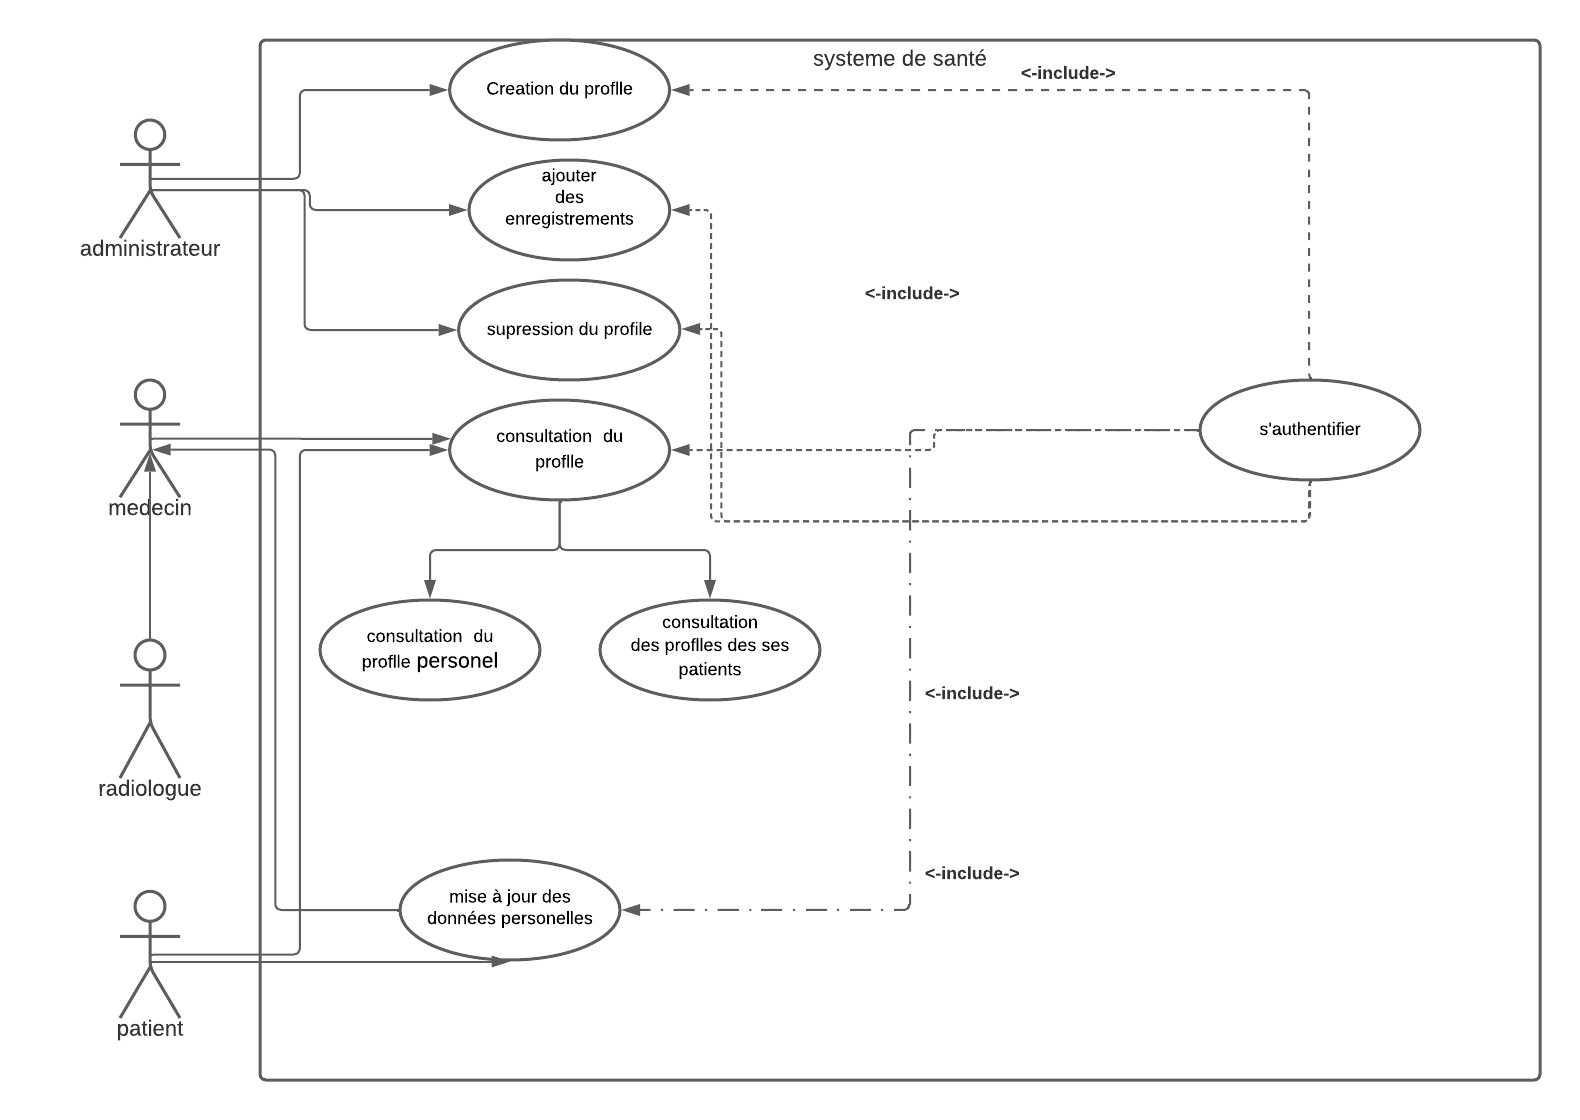
\includegraphics[height=8cm,width=18cm]{usecasediag.png}
\end{center}
\caption{Diagramme de cas d'utilisation}
\end{figure}

\subsection{Diagramme de classe}

\begin{figure}[!h]
\begin{center}
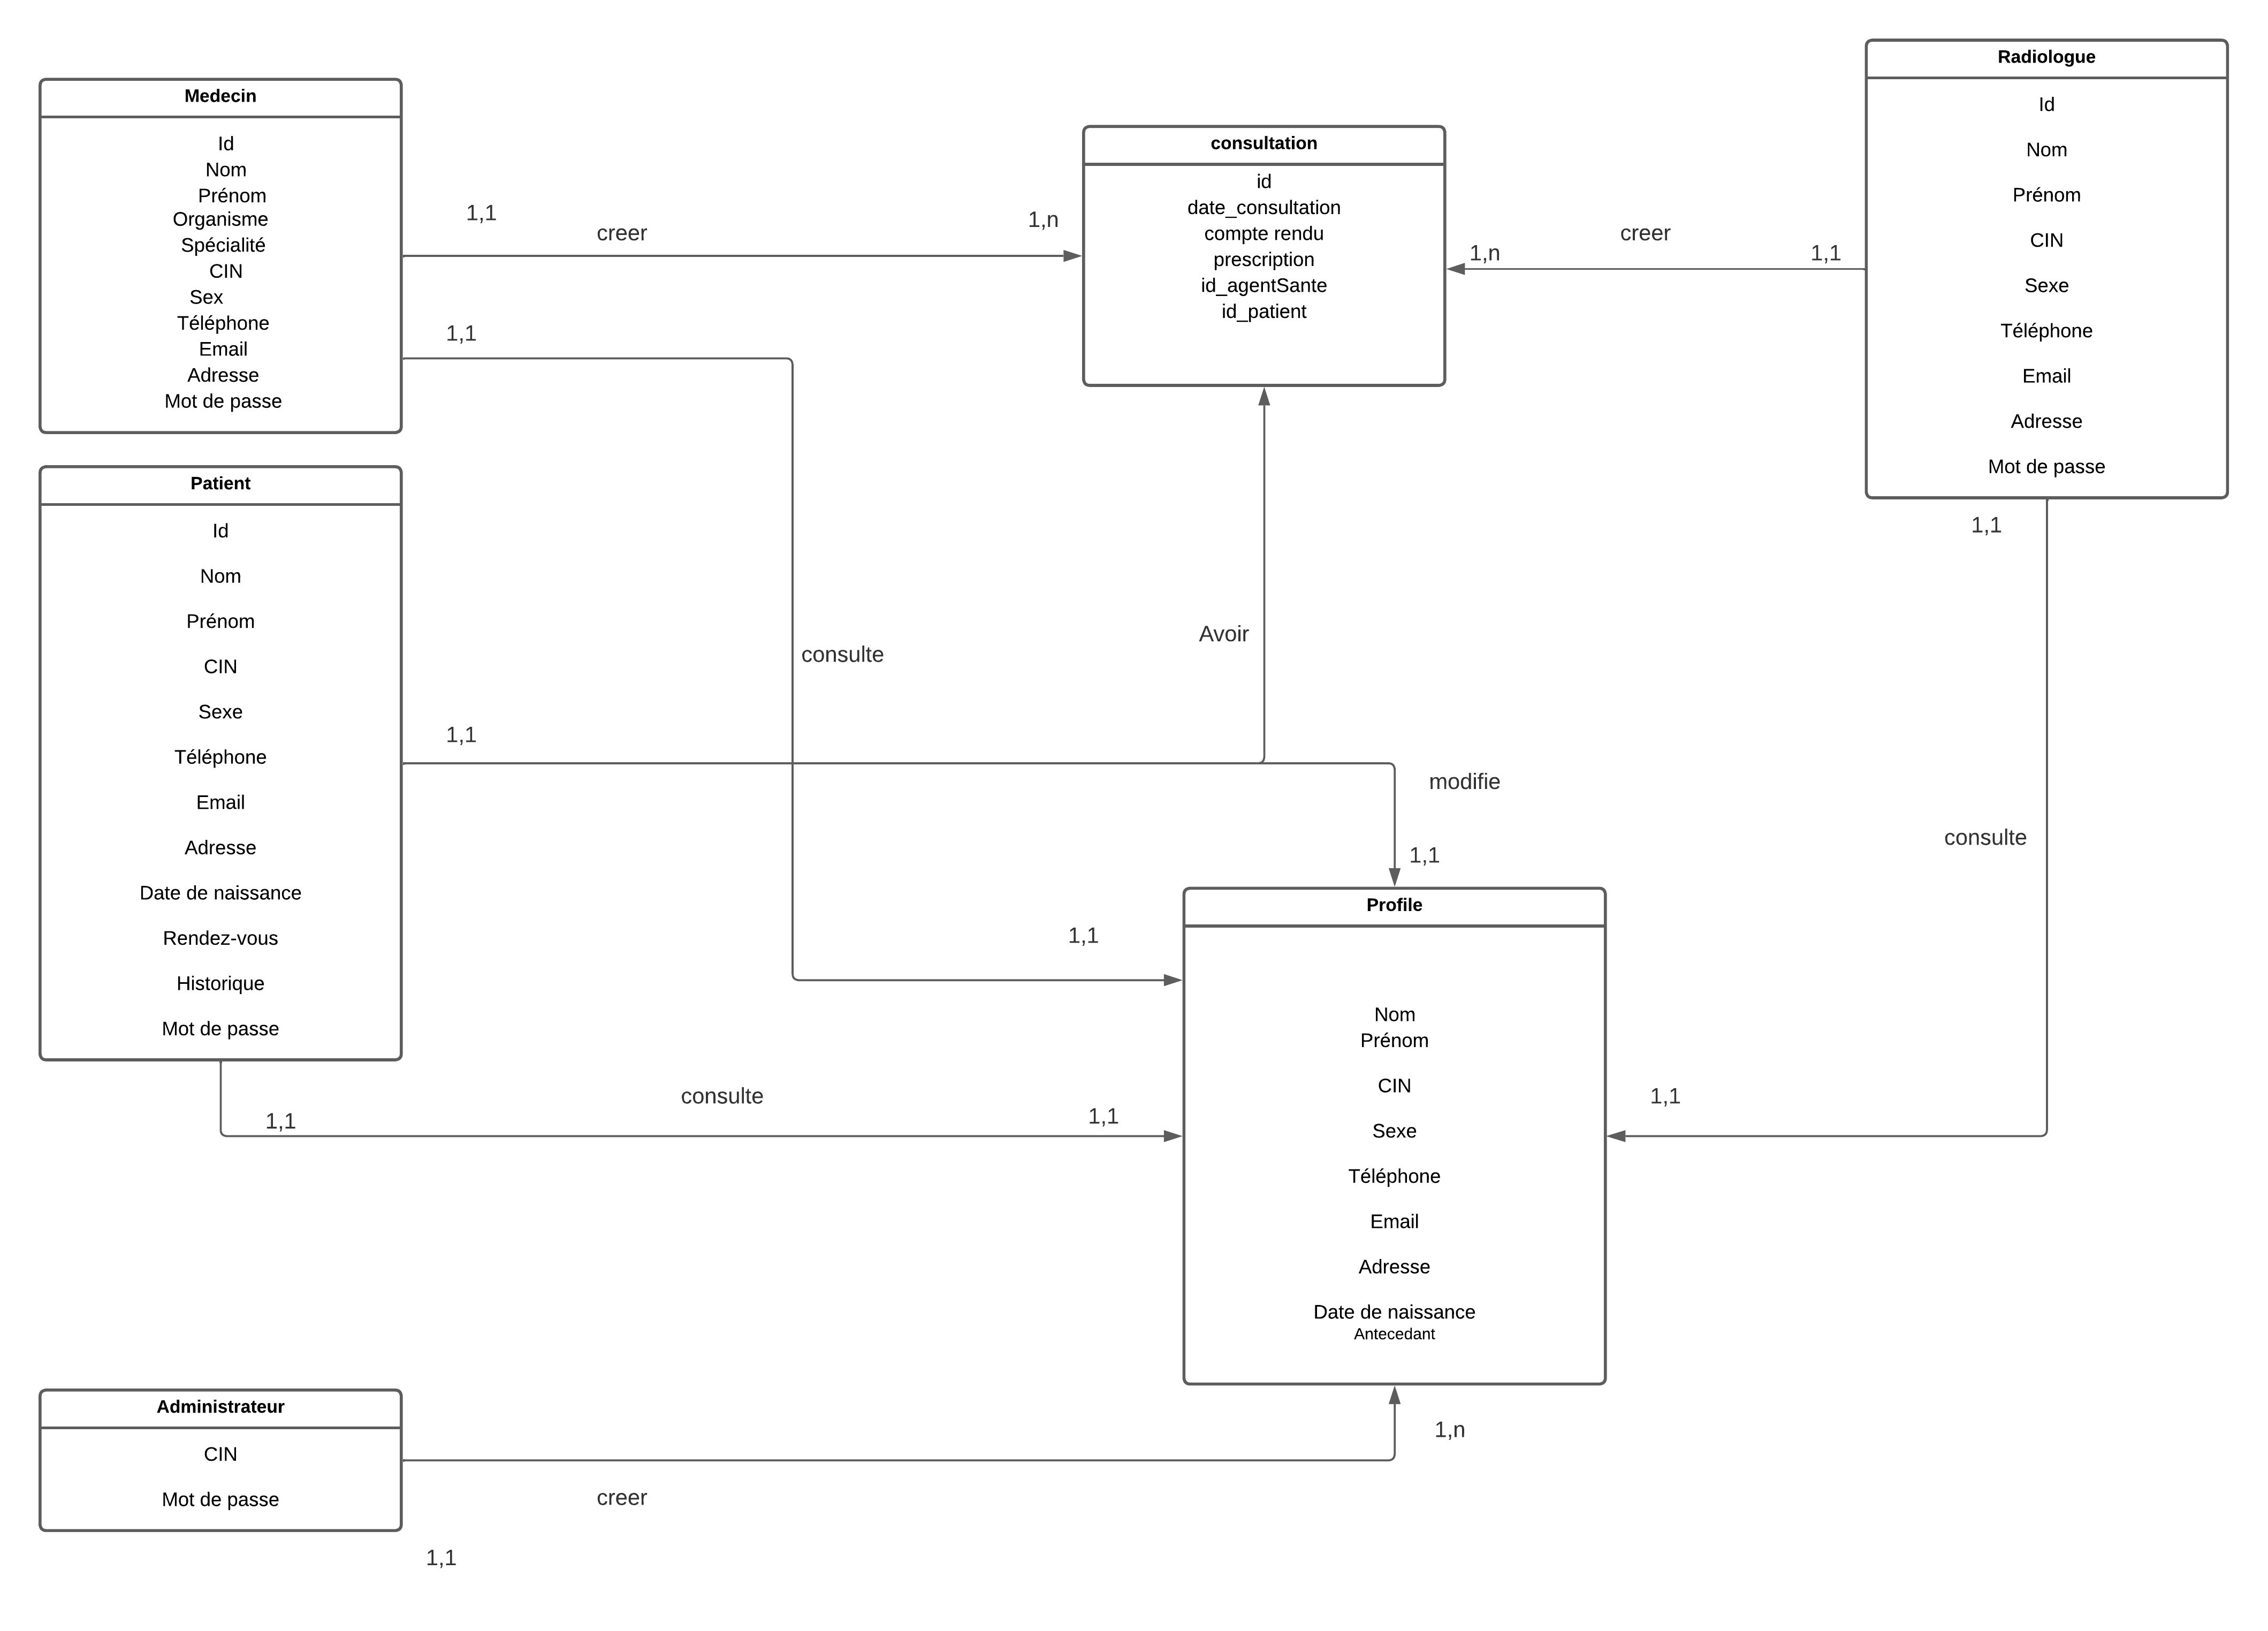
\includegraphics[height=10cm,width=18cm]{classdiag.png}
\end{center}
\caption{Diagramme de classe}
\end{figure}


\section{Conclusion} 

Aprés terminer cette étape d'analyse et conception nous avons une vision claire sur la réalisation qui est l'étape suivante qui vient aprés le choix des outils technologique.


